
\begin{figure}[H]
  {
    \setlength{\tabcolsep}{3.0pt}
    \setlength\cmidrulewidth{\heavyrulewidth} % Make cmidrule = 
    \begin{adjustbox}{height=5cm,center}
      \footnotesize
      \begin{tabular}{ll}

        \makecell[l]{
\icode{.BYTE \$00,\$01,\$01,\$02}\\
\icode{.BYTE \$00,\$FF,\$00,\$00}
} & \makecell[l]{

\includegraphics[width=1.3cm]{src/patterns/pixels/pixel_pattern11_0.png}%
} \\
        \midrule

        \makecell[l]{
\icode{.BYTE \$00,\$00,\$01,\$02,\$02}\\
\icode{.BYTE \$00,\$01,\$01,\$01,\$02}
} & \makecell[l]{

\includegraphics[width=1.3cm]{src/patterns/pixels/pixel_pattern11_1.png}%

\includegraphics[width=1.3cm]{src/patterns/pixels/pixel_pattern11_2.png}%
} \\
        \midrule

        \makecell[l]{
\icode{.BYTE \$00,\$00,\$00,\$02}\\
\icode{.BYTE \$00,\$02,\$03,\$03}
} & \makecell[l]{
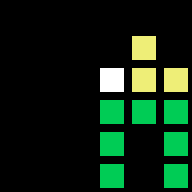
\includegraphics[width=1.3cm]{src/patterns/pixels/pixel_pattern11_3.png}%
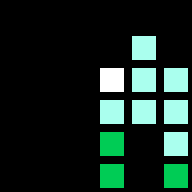
\includegraphics[width=1.3cm]{src/patterns/pixels/pixel_pattern11_4.png}%
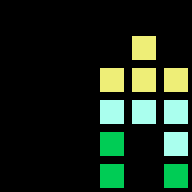
\includegraphics[width=1.3cm]{src/patterns/pixels/pixel_pattern11_5.png}%
} \\
        \midrule

        \makecell[l]{
\icode{.BYTE \$00,\$FF,\$FE}\\
\icode{.BYTE \$00,\$01,\$00}
} & \makecell[l]{
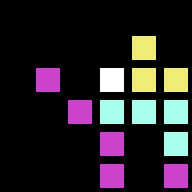
\includegraphics[width=1.3cm]{src/patterns/pixels/pixel_pattern11_6.png}%
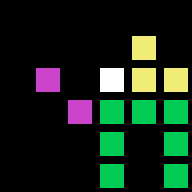
\includegraphics[width=1.3cm]{src/patterns/pixels/pixel_pattern11_7.png}%
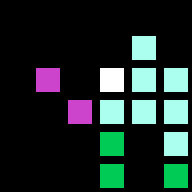
\includegraphics[width=1.3cm]{src/patterns/pixels/pixel_pattern11_8.png}%
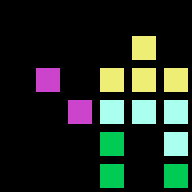
\includegraphics[width=1.3cm]{src/patterns/pixels/pixel_pattern11_9.png}%
} \\
        \midrule

        \makecell[l]{
\icode{.BYTE \$00,\$FE,\$FE}\\
\icode{.BYTE \$00,\$FF,\$FE}
} & \makecell[l]{
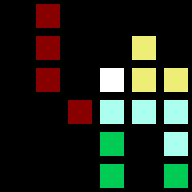
\includegraphics[width=1.3cm]{src/patterns/pixels/pixel_pattern11_10.png}%
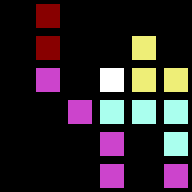
\includegraphics[width=1.3cm]{src/patterns/pixels/pixel_pattern11_11.png}%
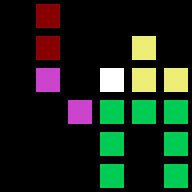
\includegraphics[width=1.3cm]{src/patterns/pixels/pixel_pattern11_12.png}%
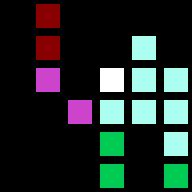
\includegraphics[width=1.3cm]{src/patterns/pixels/pixel_pattern11_13.png}%
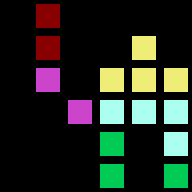
\includegraphics[width=1.3cm]{src/patterns/pixels/pixel_pattern11_14.png}%
} \\
        \midrule

        \makecell[l]{
\icode{.BYTE \$00,\$FD,\$FE}\\
\icode{.BYTE \$00,\$FF,\$FF}
} & \makecell[l]{
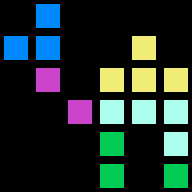
\includegraphics[width=1.3cm]{src/patterns/pixels/pixel_pattern11_15.png}%
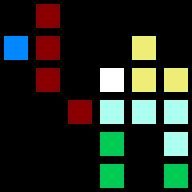
\includegraphics[width=1.3cm]{src/patterns/pixels/pixel_pattern11_16.png}%
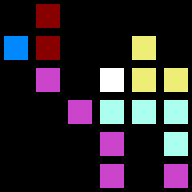
\includegraphics[width=1.3cm]{src/patterns/pixels/pixel_pattern11_17.png}%
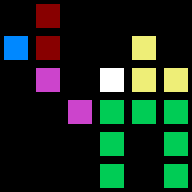
\includegraphics[width=1.3cm]{src/patterns/pixels/pixel_pattern11_18.png}%
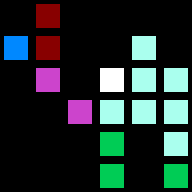
\includegraphics[width=1.3cm]{src/patterns/pixels/pixel_pattern11_19.png}%
} \\
        \midrule

        \makecell[l]{
\icode{.BYTE \$00}\\
\icode{.BYTE \$00}
} & \makecell[l]{
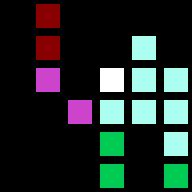
\includegraphics[width=1.3cm]{src/patterns/pixels/pixel_pattern11_20.png}%
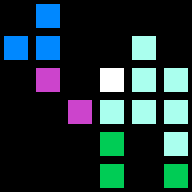
\includegraphics[width=1.3cm]{src/patterns/pixels/pixel_pattern11_21.png}%
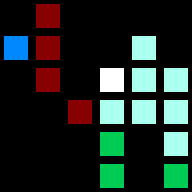
\includegraphics[width=1.3cm]{src/patterns/pixels/pixel_pattern11_22.png}%
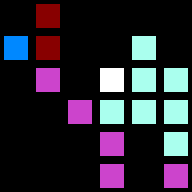
\includegraphics[width=1.3cm]{src/patterns/pixels/pixel_pattern11_23.png}%
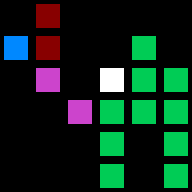
\includegraphics[width=1.3cm]{src/patterns/pixels/pixel_pattern11_24.png}%
} \\
        \midrule

      \end{tabular}
    \end{adjustbox}
  }\caption{The purpose of each of the oscillator values.}
\end{figure}
